
\chapter{太陽光発電データの時刻補正手法}
\label{chap:second}

\section{緒言}
本章では太陽光発電データの時刻補正手法について述べる.

% 20220523

\section{太陽光発電の計測データの問題点について}
CSVデータなどで保存された太陽光発電の環境データはオフライン環境でファイル書き込みを行っているため, PCの内部時計がずれており, 計測データの日時情報が正確な日時とは異なっている.

そこで相互相関を用いて, 実測した日射量の時系列データと, 計算式により求まる日射量の時系列データとの時間的遅延の秒数を検出することで, 実測データの計測日時のずれ時間を推定する.

\section{大気外全天日射量の計算式}
任意の緯度経度, 日時における日射量$Q$は, 任意の緯度$\phi$, 経度$\lambda$の地点における任意の日時, 太陽高度$\alpha$から求めることができる.

まず, 次式により元旦からの通し日数$dn$に基いて定めた$\theta$を用いて, 当該日の太陽赤緯$\delta$, 地心太陽距離$\frac{r}{r^{*}}$, 均時差$E_q$をそれぞれ以下の式により求める.
\begin{eqnarray}
  \theta =  \frac{2\pi (dn-1)}{365}
\end{eqnarray}

\begin{eqnarray}
  \begin{split}
    \delta =  0.006918-0.399912\cos \theta+0.070257\sin \theta-0.006758\cos 2\theta\\
    +0.000907\sin 2\theta-0.002697\cos 3\theta+0.001480\sin 3\theta
  \end{split}
\end{eqnarray}

\begin{dmath}
  \frac{r}{r^{*}} =  \frac{1}{\sqrt{1.000110+0.034221\cos \theta+0.001280\sin \theta+0.000719\cos 2\theta+0.000077\sin 2\theta}}
\end{dmath}

\begin{eqnarray}
  \begin{split}
    E_q =  0.000075+0.001868\cos \theta-0.032077\sin \theta\\
    -0.014615\cos 2\theta-0.040849\sin 2\theta
  \end{split}
\end{eqnarray}

日本標準時間から, 太陽の時角$h$を求める.

\begin{eqnarray}
  h = \frac{(日本標準時間-12)\pi}{12}+標準子午線からの経度差+E_q
\end{eqnarray}

$\delta$, $\phi$, $h$の値が既知となったので$\alpha$は

\begin{eqnarray}
  \alpha = \arcsin (\sin \phi\sin \delta+\cos \phi\cos \delta\cos h)
\end{eqnarray}

として求めることができる.

最後に, $Q$を

\begin{eqnarray}
  Q = 1367(\frac{r^{*}}{r})^{2}\sin \alpha
\end{eqnarray}

により求めることができる.
また, 1367\si{\watt}/\si{\metre\squared}は太陽定数である.

式(2.1)~式(2.7)を用いることで, 任意の緯度経度, 日時における日射量が求まる.

% 20220529

\section{実測データと大気外全天日射量との比較}
Elasticsearchサーバーから取得した日射量データと, 計算式から求めた大気外全天日射量をプロットしたものを図\ref{20220529-p1}に示す.
図\ref{20220529-p1}はElasticsearchサーバーから取得した2022年6月2日の日射量データと, リサイクル館の緯度経度と日付情報より求めた大気外全天日射量の値をプロットしている.

\begin{figure}[h]
  \begin{center}
    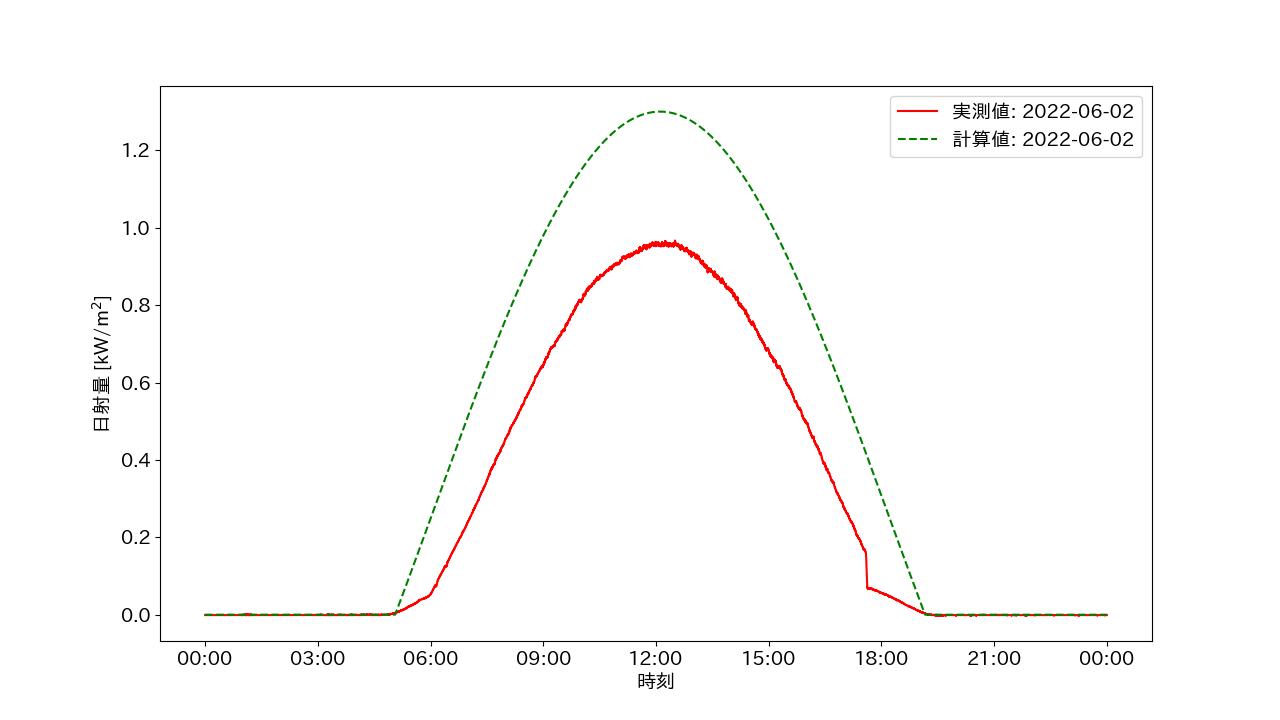
\includegraphics[width=160mm]{sotu/figure/2/original-20220602-corr.png}
    \caption{2022年6月2日の日射量の実測データと大気外全天日射量をプロットしたもの}
    \label{20220529-p1}
  \end{center}
\end{figure}

% 20220620

\section{相互相関によるずれ時間の推定}
今回, 相互相関の計算に使用する実測データの範囲を, 2022年6月2日0時0分から2022年6月2日23時59分まで期間とする.

2022年6月2日を選定した理由は, 図\ref{20220529-p1}より, 2022年6月2日の実測データの概形は大気外全天日射量の概形と類似していたためである.

実測データの計測日時の情報をもとに, 大気外全天日射量を求め, これらの値を入力として相互相関を計算する.

相互相関の計算結果より, 大気外全天日射量の日時を実測データより124秒進めた際に, 相互相関の値が最大となった.

しかし, 今回使用した実測データには計測日時のずれは殆どないため, 大気外全天日射量の日時を進めていない際に実測データとの相関が最大となるのが正しい.

これは, 日射量の計算式の予測精度が低いことが原因であると考えられる.

\section{地表日射量の予測}

日射量の予測精度を改善するため, 式(2.1)~式(2.7)を使った方法ではなく, pvlibというライブラリを使用して, 地表日射量を求めることで相互相関を計算する.

\section{pvlibの概要}
pvlibは, 太陽光発電システムの性能シミュレーションや関連するタスクを実行するための関数とクラスのセットを提供する, コミュニティが開発したツールボックスである. 

以下は, pvlibの主な特徴である.

\begin{itemize}
  \item 太陽位置計算: pvlibは, 地球上の任意の場所における太陽の位置を計算する機能を提供する. これは, 太陽の方位角や高度角を求めるのに使用される.
  \item 大気透過モデル: 大気を通過する太陽放射の量や質を推定するモデルが含まれている.
  \item 太陽光発電システムの性能モデリング: 太陽光発電モジュールやインバーターの性能モデルが含まれており, 異なる条件下での太陽光発電システムの出力をシミュレートできる.
\end{itemize}

\section{実測データとpvlibによる地表日射量の比較}
Elasticsearchサーバーから取得した日射量データと, pblivを用いて求めた地表日射量をプロットしたものを図\ref{2-p1}に示す.
図\ref{2-p1}はElasticsearchサーバーから取得した2022年6月2日の日射量データと, リサイクル館の緯度経度と日付情報を入力としてpvlibより求めた地表日射量をプロットしている.

図\ref{20220529-p1}と比較して, pvlibより求めた地表日射量が実測データにより近い概形となっていることが分かる.

\begin{figure}[h]
  \begin{center}
    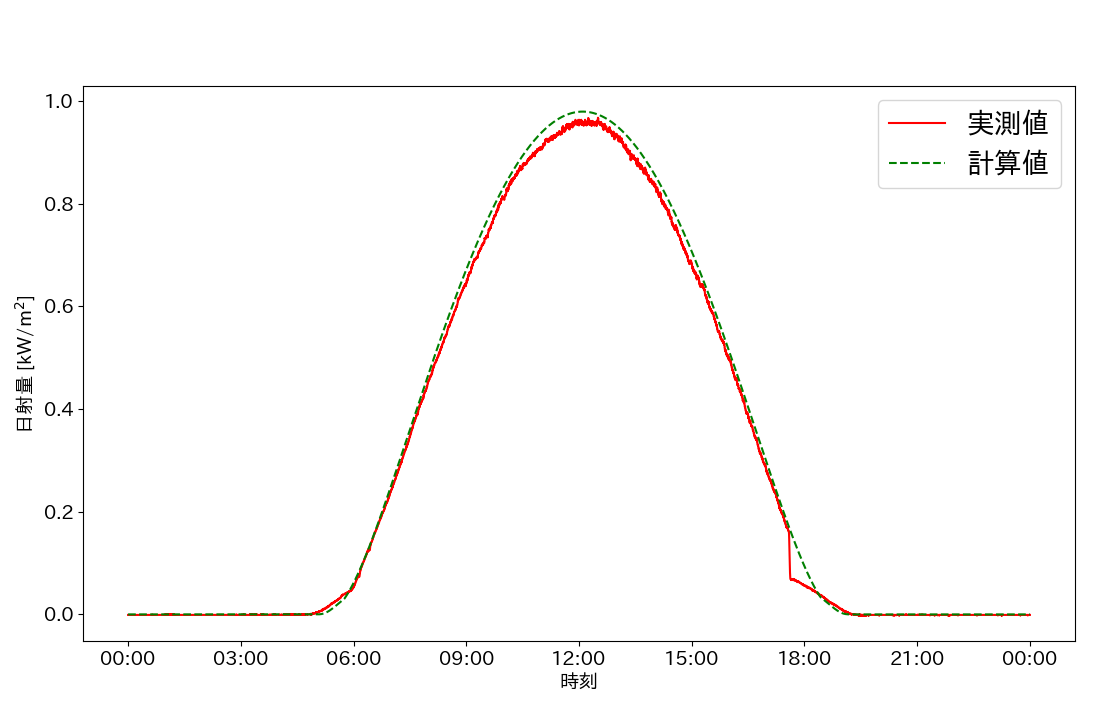
\includegraphics[width=160mm]{sotu/figure/2/pvlib-20220602-corr.png}
    \caption{2022年6月2日の実測データと地表日射量をプロットしたもの}
    \label{2-p1}
  \end{center}
\end{figure}

\section{地表日射量との相互相関によるずれ時間の推定}
相互相関の計算に使用する実測データの範囲を, 2022年6月2日0時0分から2022年6月2日23時59分まで期間とする.

実測データの計測日時の情報をもとに, pvlibより地表日射量を求め, これらの値を入力として相互相関を計算する.

相互相関を求めた結果, 地表日射量の日時を実測データより74秒進めた際に, 相互相関の値が最大となることが分かった.

式(2.1)~式(2.7)を用いて求めた大気外全天日射量データ用いて相互相関を計算した時と比較して, 124秒から74秒へと50秒改善した.

\section{前処理の追加によるずれ時間推定精度改善}

図\ref{2-p1}では, 日没の辺りにおいて, 実測データと地表日射量の概形が大きくことなっている.

このような実測データに影響を与える外部要因を事前に除去した上で, 相互相関を計算する前処理を追加することで相互相関の計算結果が改善するか検証する.

前処理を含めた相互相関の計算方法は以下のステップで行う.

\begin{enumerate}
  \item 実測データの日射量を0 \si{\kilo\watt}/\si{\metre\squared}と見なすしきい値の指定: まず, 実測データをフィルタリングするために日射量のしきい値を設定する. 今回は, q=0.2 \si{\kilo\watt}/\si{\metre\squared}をしきい値として設定する.
  \item しきい値に該当するタイムスタンプの推定: 続いて, 実測データの各データ点から0.2 \si{\kilo\watt}/\si{\metre\squared}を減算して絶対値を取った際に最も0に近い値を取るタイムスタンプを午前と午後でそれぞれ一点ずつ推定する.
  \item 推定したタイムスタンプを使った実測データのフィルタリング: 前のステップで得たタイムスタンプを使用して, 2点のタイムスタンプの外側にある実測データの日射量を0 \si{\kilo\watt}/\si{\metre\squared}とする.
  \item 地表日射量との相互相関の計算: 実測データをフィルタリングした後, 地表日射量との相互相関を計算する.
\end{enumerate}

図\ref{2-p2}に上述の前処理によってフィルタリングされた実測データと, 地表日射量をプロットしたものを示す.

\begin{figure}[h]
  \begin{center}
    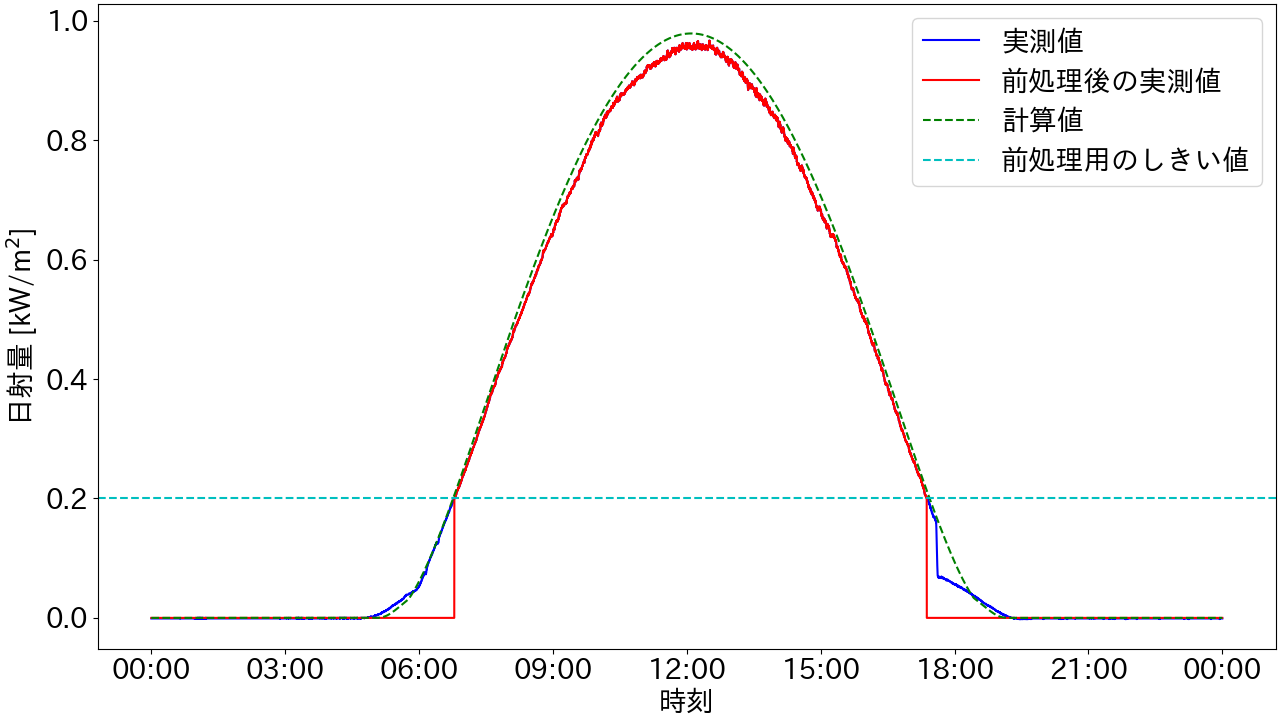
\includegraphics[width=160mm]{sotu/figure/2/drop-under-0.2-q.png}
    \caption{前処理によってフィルタリングされた実測データと, 地表日射量をプロットしたもの}
    \label{2-p2}
  \end{center}
\end{figure}

図\ref{2-p2}にプロットしたフィルタリングされた実測データと, 地表日射量を入力として相互相関を計算する.

相互相関を求めた結果, 地表日射量の日時を実測データより27秒進めた際に, 相互相関の値が最大となることが分かった.

pvlibを使って求めた日射量データを入力として相互相関を計算した時と比較して, 74秒から27秒へと47秒改善した.

\section{結言}
本章では太陽光発電データの時刻補正手法について述べた. 
次章では学内ゾーンで稼働している Elasticsearch クラスタへのデータ移行について述べる.